\documentclass[12pt,a4paper]{article}
\usepackage{fontspec}
\usepackage{polyglossia}
\setdefaultlanguage{russian}
\setotherlanguage{english}
\setmainfont{STIX Two Text}[AutoFakeBold=1.5]
\setmonofont{Menlo}
\newfontfamily\cyrillicfonttt{Menlo}
\usepackage[a4paper,margin=2cm]{geometry}
\usepackage{graphicx}
\usepackage{longtable,tabularx,array,booktabs}
\usepackage{float,caption,enumitem,pdflscape,xurl,listings}
\usepackage{hyperref}
\usepackage{etoolbox}
\hypersetup{colorlinks=true,linkcolor=blue,urlcolor=blue}
\setlength{\parindent}{1.25cm}
\setlength{\parskip}{0.25em}
\renewcommand{\arraystretch}{1.16}
\setlist{nosep,leftmargin=1.5em}
\lstset{basicstyle=\ttfamily\footnotesize,breaklines=true,columns=fullflexible,frame=single,keepspaces=true,showstringspaces=false}
\AtBeginEnvironment{longtable}{\small}
\sloppy
\begin{document}
\begin{titlepage}
\centering
{\large Практическая работа\par}
\vspace{2.5cm}
{\LARGE\bfseries Отчёт по практической работе № 4\par}
\vspace{0.6cm}
{\Large Проектирование защищённой архитектуры приложения\par}
\vspace{1.8cm}
\begin{tabular}{p{4cm}p{11cm}}
Дисциплина: & Основы разработки защищённого программного обеспечения и компьютерных сетей\\
Вариант: & 19 - Система учёта транспортных средств организации\\
Исходная версия: & v0.3\\
Версия работы: & v0.4 - Secure Architecture\\
Студент: & Мостовая Полина Андреевна\\
Группа: & ИУСбд-02-23
\end{tabular}
\vfill
{\large 2026\par}
\end{titlepage}
\tableofcontents
\clearpage

\section{Цель работы}
Спроектировать архитектуру защиты для системы учёта транспортных средств, связать компоненты с угрозами v0.3 и реализовать небольшой проверяемый прототип: предметную валидацию, контроль ролей и объектов, сервисную операцию и аудит. Результат должен отделять действующие проверки от проектных механизмов. Подход продолжает методические указания работы № 4 \cite{method4}.

\section{Исходное состояние и предметная область}
Проект варианта 19 предназначен для ведения реестра автопарка, назначений, поездок, пробега, неисправностей, обслуживания и отчётности. В исходном commit версии v0.3 приложение загружало и проверяло настройки \texttt{APP\_NAME}, \texttt{APP\_ENV}, \texttt{APP\_SECRET\_KEY}, затем печатало безопасное стартовое сообщение. Было три теста. Полноценной аутентификации, веб/API-интерфейса, базы данных, учёта ТС и поездок и аудита не было.

v0.4 сохраняет \texttt{app.main} и \texttt{app.config}, добавляя модули валидации, авторизации, аудита и учебные сервисные операции над in-memory данными. В проекте нет СУБД, сетевого интерфейса или реального входа пользователя. Архитектура и тесты сверены с практической работой №4, отчётами №2–3 и фактическим состоянием репозитория.

\section{Активы и выбранные угрозы}
К ключевым активам относятся \texttt{AS-2} профили и роли, \texttt{AS-3} конфигурация и секрет, \texttt{AS-4} реестр ТС, \texttt{AS-5} назначения и поездки, \texttt{AS-6} техническое состояние и \texttt{AS-7} аудит. Сохранены значения ID и связи из предыдущих работ.

\begin{longtable}{p{1.7cm}p{4.5cm}p{2cm}p{2.4cm}p{3.5cm}}
\caption{Угрозы v0.3, включённые в анализ v0.4}\\
\toprule ID & Сценарий & Активы & Риск до мер & Статус\\\midrule\endfirsthead
\toprule ID & Сценарий & Активы & Риск до мер & Статус\\\midrule\endhead
TH-01 / RS-01 & Подбор учётных данных сотрудника & AS-1, AS-2 & L=3, S=2, R=6 & Мера проектируется\\
TH-03 / RS-03 & Фиктивная выдача/смена ответственного & AS-2, AS-5 & L=2, S=2, R=4 & Назначения не реализованы\\
TH-04 / RS-04 & Некорректная карточка или статус ТС & AS-4, AS-6 & L=2, S=2, R=4 & Частичная проверка\\
TH-05 / RS-05 & Подмена пробега/отчёта & AS-5 & L=2, S=2, R=4 & Валидация реализована\\
TH-06 / RS-06 & Повышение роли через запрос & AS-2 & L=2, S=3, R=6 & Авторизация прототипа проверена\\
TH-07 / RS-07 & Отрицание изменения роли & AS-2, AS-7 & L=1, S=3, R=3 & Аудит частичный\\
TH-08 / RS-08 & Чтение чужого маршрута & AS-5, AS-8 & L=3, S=3, R=9 & Объектный отказ проверен\\
TH-09 / RS-09 & Утечка секрета через диагностику & AS-3 & L=1, S=2, R=2 & Штатный вывод безопасен\\
\bottomrule
\end{longtable}
Оценки \texttt{R=L×S} перенесены из исходного реестра, а не пересчитаны по результатам unit-тестов. Проектное снижение баллов риска не объявляется достигнутым.

\section{Архитектурные компоненты и границы}
Архитектура - небольшой модульный монолит с отдельными обязанностями: CLI/вход, Validation, Authentication, Authorization, Services, Repository, Storage, Audit и Configuration. Validation, Authorization, Audit и Configuration имеют код; сервисы реализованы только для демонстрационного потока. Authentication и Repository проектируются, долговременное Storage отсутствует.

Фактические точки входа: запуск конфигурации командой \texttt{python -m app.main}; демонстрационные команды \texttt{python -m app.demo} с параметрами \texttt{--validation} и \texttt{--authorization}; переменные окружения и локальный \texttt{.env}. Веб-формы, API, загрузка файлов и подключение к СУБД не реализованы и не открыты. Параметры demo передаются вызовам Python-сервиса, а не принимаются как аутентифицированная роль от клиента.

\begin{longtable}{p{2.0cm}p{4.0cm}p{9.2cm}}
\caption{Границы доверия и контроль}\\
\toprule ID & Поток & Контроль\\\midrule\endfirsthead
\toprule ID & Поток & Контроль\\\midrule\endhead
TB-01 & Клиент -- приложение & Ввод недоверенный; проверка типа/границ данных, затем trusted principal, роль и объект. Реального HTTP-клиента нет.\\
TB-02 & Приложение -- хранилище & В будущей СУБД - доступ сервисов через repository и минимальные права; сейчас работает только память процесса.\\
TB-03 & Приложение -- аудит & Событие фиксированного формата без пароля, секрета и маршрута; ограничение доступа и ротация пока проектируются.\\
\bottomrule
\end{longtable}

\section{Архитектурная схема}
Схема различает реализованные, частично реализованные и проектируемые группы. Входы окружения, CLI и будущие операции показаны отдельно.
\clearpage
\begin{landscape}
\thispagestyle{empty}
\begin{figure}[p]
\centering
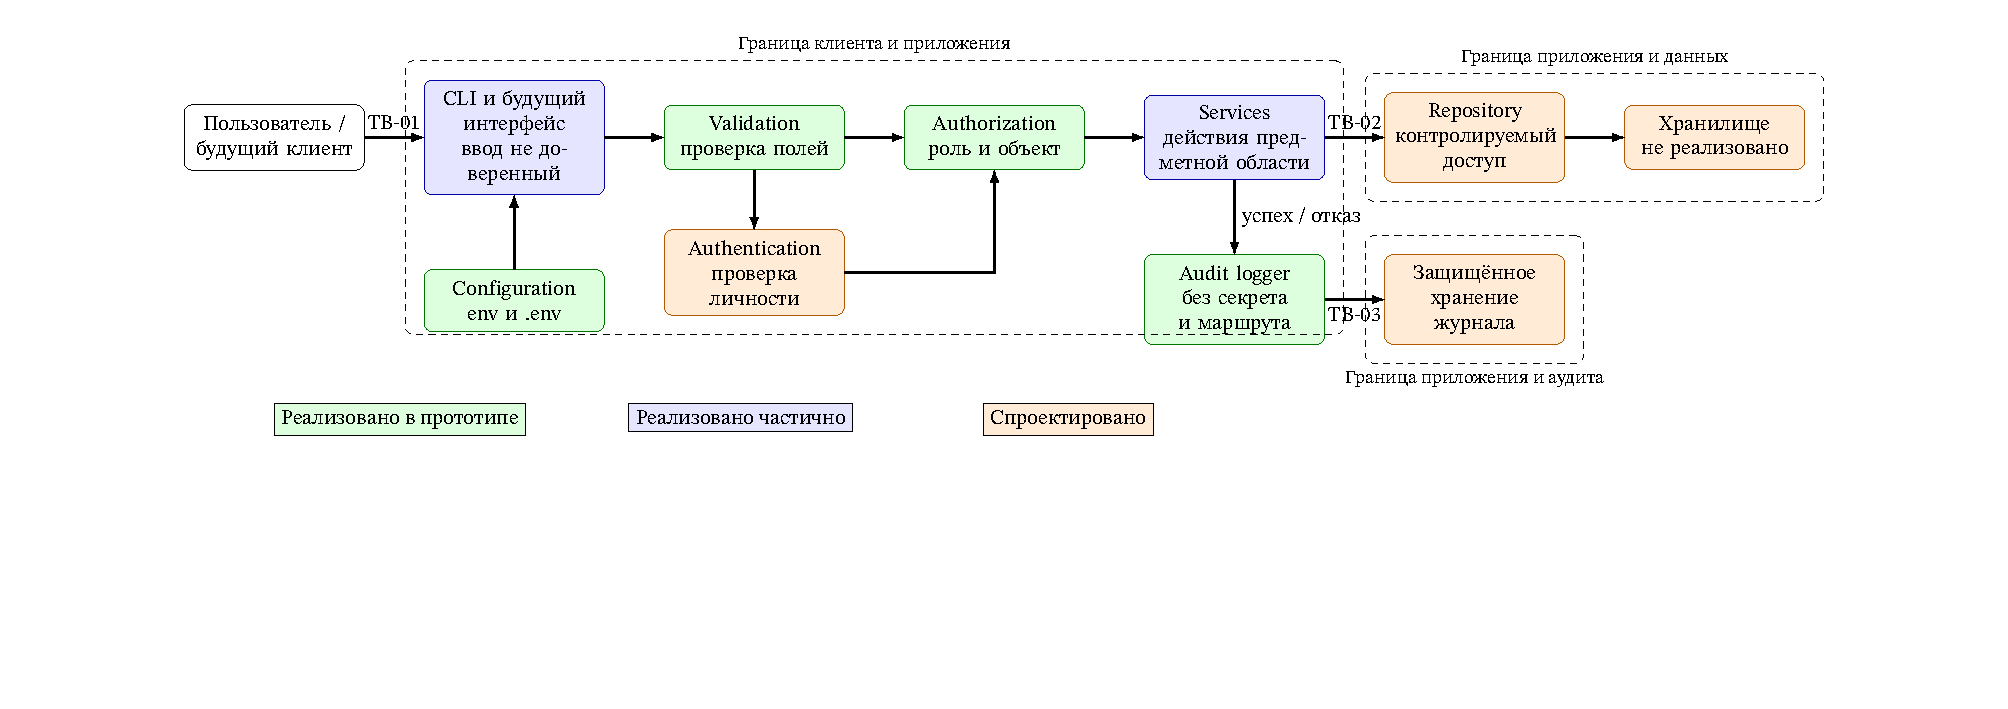
\includegraphics[width=0.85\paperheight,trim=2.2cm 4.2cm 2.2cm 0cm,clip,keepaspectratio]{figures/secure_architecture.pdf}
\caption{Защищённая архитектура системы учёта транспортных средств v0.4.}
\end{figure}
\end{landscape}
\clearpage
Редактируемый исходник схемы находится в \texttt{docs/secure\_architecture.mmd}, векторный экспорт -- в \texttt{reports/lab4/figures/secure\_architecture.pdf}.

\section{Модель доступа и аутентификация}
Аутентификация не реализована. Для будущего серверного интерфейса проектируются verifier пароля вместо исходного пароля, ограничение повторных попыток, выдача и отзыв сеансов, а также серверное создание доверенного контекста. Демонстрационный \texttt{Principal} - искусственный контекст теста; значение роли от клиента не может считаться доказательством личности.

\begin{longtable}{p{3.2cm}p{2.2cm}p{2.2cm}p{2.2cm}p{3.6cm}}
\caption{Сокращённая матрица разрешений}\\
\toprule Операция & Водитель & Диспетчер & \shortstack{Руководи-\\тель} & \shortstack{Администратор\\безопасности}\\\midrule\endfirsthead
\toprule Операция & Водитель & Диспетчер & \shortstack{Руководи-\\тель} & \shortstack{Администратор\\безопасности}\\\midrule\endhead
Смена состояния ТС & Запрет & Разрешено & Запрет & Запрет\\
Чтение поездки & Только назначенная & По служебной задаче & Запрет & Запрет\\
Сводный отчёт & Запрет & По служебной задаче & Только агрегат & Запрет\\
Чтение аудита & Запрет & Запрет & Запрет & Разрешено\\
Управление ролями & Запрет & Запрет & Запрет & Разрешение по процедуре\\
\bottomrule
\end{longtable}
Неаутентифицированный субъект не получает защищённые полномочия. Неизвестная роль и неизвестная операция запрещаются. Администратор безопасности не получает автоматическое чтение маршрутов.

\section{Валидация, конфигурация и аудит}
Модуль валидации проверяет единый формат ASCII-идентификаторов ТС и поездки длиной до 32 символов, допустимые статусы ТС, целочисленный неотрицательный пробег, монотонность показаний и описание дефекта не длиннее 500 символов. Верхний предел километров не придумывается. Ошибка возникает до изменения in-memory состояния. Поскольку в предыдущих требованиях нет таблицы переходов статусов, прототип проверяет допустимое конечное значение, но не вводит дополнительные правила переходов.

Конфигурация наследуется из v0.3: переменные окружения/локальный \texttt{.env}; имя и режим проверяются; \texttt{APP\_SECRET\_KEY} не короче 32 символов; \texttt{.env} исключён Git, пример содержит placeholder. Ошибочное значение приводит к отказу при запуске.

Аудит содержит UTC-время, субъект, действие, объект и исход. Допустимые действия и результаты ограничены списком, идентификаторы проходят форматную проверку; успехи, отказы и ошибки валидации фиксируются через \texttt{logging}. Модуль не настраивает глобальный root logger при импорте и не получает секреты или подробности поездки. Долговременная защита и политика хранения не реализованы.

\section{Матрица угроз и защит}
\begin{landscape}
\begin{longtable}{p{1.8cm}p{3.5cm}p{3.5cm}p{6cm}p{6.2cm}}
\caption{Угроза - компонент - защита - остаточный риск}\\
\toprule № / угроза & Компонент & Механизм & Почему снижает риск & Остаточный риск\\\midrule\endfirsthead
\toprule № / угроза & Компонент & Механизм & Почему снижает риск & Остаточный риск\\\midrule\endhead
1 TH-01 & Authentication & Лимит попыток и отзыв сеанса (проект) & Снижает возможность повторного подбора и срок использования чужого сеанса & Входа и лимита нет; не проверено\\
2 TH-03 & Service, repository & Допустимые переходы и история ответственного (проект) & Запрещает недопустимые изменения и сохраняет причину/субъекта & Назначения не реализованы\\
3 TH-04 & Validation, authorization & Проверка статуса и роль диспетчера & Неподходящее поле отклоняется до изменения; тест фиксирует отсутствие мутации & Прототип обрабатывает лишь статус одного ТС\\
4 TH-05 & Validation, authorization & Монотонность пробега; сверка владельца поездки & Отсекает отрицательное/обратное показание и чужой объект & Нет сохранения отчёта или БД\\
5 TH-06 & Authorization & Явный список прав, deny by default & Запрос не расширяет серверную роль; негативные роли проверены тестами & Нет реальной аутентификации\\
6 TH-08 & Authorization, service & Сверка владельца поездки до выдачи объекта & Чужой водитель получает отказ до возврата записи & Проверено только на объекте памяти\\
7 TH-09 & Configuration, audit & Безопасное стартовое сообщение и фиксированный формат аудита & Секрет и содержимое поездки не передаются логгеру & Инфраструктурная диагностика не проверена полностью; SEC-9/SEC-10, AT-15\\
8 TH-07 & Audit & Субъект, действие, объект, время и исход & Запись позволяет наблюдать зафиксированный исход операции & Нет неизменяемого долговременного журнала\\
\bottomrule
\end{longtable}
\end{landscape}

\section{Структура проекта и исходный код}
\begin{lstlisting}
app/
  config.py, main.py, demo.py
  security/validation.py, access_control.py
  services/vehicle_service.py
  audit/audit_logger.py
tests/
  test_main.py, test_validation.py, test_access_control.py,
  test_audit_logger.py, test_secure_flow.py
docs/secure_architecture.md, docs/secure_architecture.mmd
reports/lab4/report.tex, report.pdf, figures/, screenshots_manual/
\end{lstlisting}

Ниже включены полные исходники трёх требуемых модулей и сервисной связки из рабочей копии.
\subsection{\texttt{app/security/validation.py}}
\lstinputlisting[language=Python]{../../app/security/validation.py}
\subsection{\texttt{app/security/access\_control.py}}
\lstinputlisting[language=Python]{../../app/security/access_control.py}
\subsection{\texttt{app/audit/audit\_logger.py}}
\lstinputlisting[language=Python]{../../app/audit/audit_logger.py}
\subsection{\texttt{app/services/vehicle\_service.py}}
\lstinputlisting[language=Python]{../../app/services/vehicle_service.py}

\section{Тестирование и демонстрация}
Исходный набор включал три теста. Полный набор выполнен на Python 3.12.14 командой \texttt{./.venv/bin/python -m pytest -q}: результат — 45 passed, без пропусков и ошибок. Дополнительно проверены штатный запуск \texttt{app.main} и демонстрация \texttt{app.demo}. Снимки 1–4 показывают фактический запуск, весь набор тестов, валидацию, разрешённую и запрещённую операции, неизменность данных после отказа и связанные события аудита.

\begin{longtable}{p{4cm}p{3cm}p{5.4cm}p{2.1cm}}
\caption{Проверочные сценарии}\\
\toprule Сценарий & Операция & Фактический результат & Статус\\\midrule\endfirsthead
\toprule Сценарий & Операция & Фактический результат & Статус\\\midrule\endhead
Корректное значение & Статус ТС и пробег & Валидные данные приняты & Пройдено\\
Некорректные данные & Пустой ID, неверный тип, отрицательный/обратный пробег & Контролируемый ValidationError & Пройдено\\
Административный отказ & Водитель меняет статус ТС & Отказ; статус не изменился & Пройдено\\
Запись отказа & Попытка водителя изменить ТС & В аудите \texttt{result=denied} & Пройдено\\
Объектная проверка & Чужой водитель читает поездку & AccessDenied, запись не возвращена & Пройдено\\
Отсутствие маршрута в логе & Владелец читает поездку & Аудит не содержит route & Пройдено\\
\bottomrule
\end{longtable}

\begin{figure}[H]
\centering
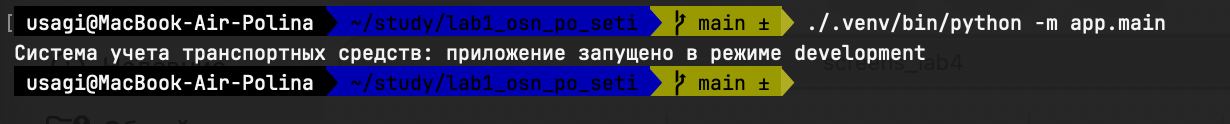
\includegraphics[width=0.97\linewidth]{screenshots_manual/lab4_1.png}
\caption{Штатный запуск приложения с загрузкой конфигурации без вывода секрета.}
\end{figure}
\begin{figure}[H]
\centering
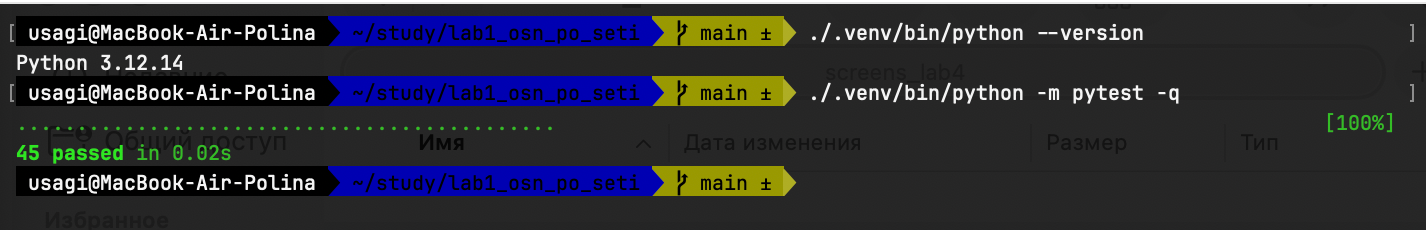
\includegraphics[width=0.97\linewidth]{screenshots_manual/lab4_2.png}
\caption{Полный запуск pytest: 45 тестов пройдены.}
\end{figure}
\begin{figure}[H]
\centering
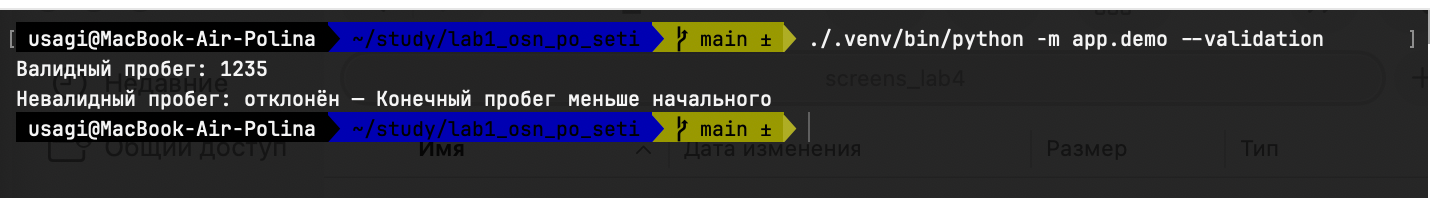
\includegraphics[width=0.97\linewidth]{screenshots_manual/lab4_3.png}
\caption{Результаты проверки корректного и некорректного пробега.}
\end{figure}
\begin{figure}[H]
\centering
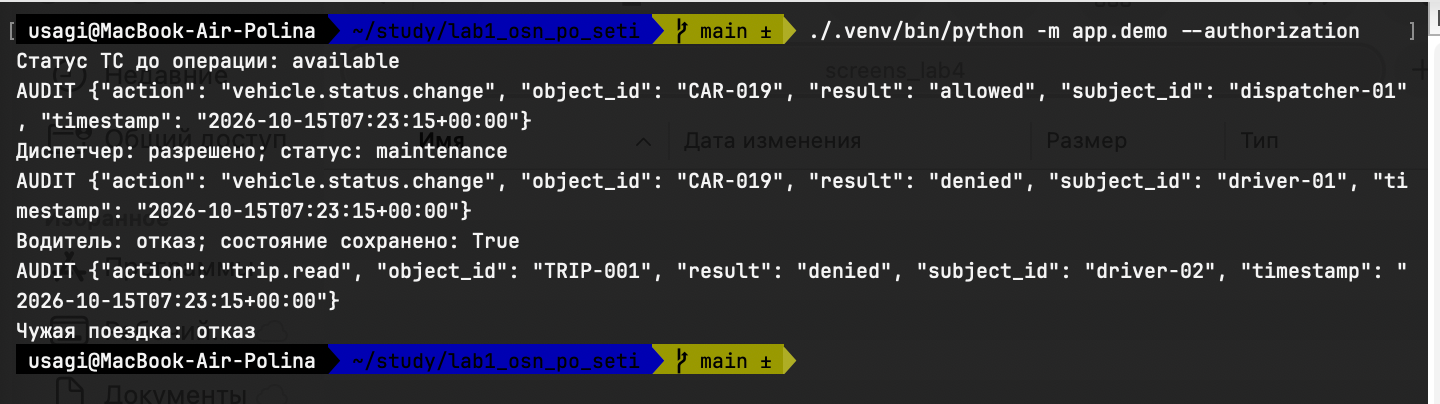
\includegraphics[width=0.97\linewidth]{screenshots_manual/lab4_4.png}
\caption{Разрешение диспетчеру, отказ водителю без изменения состояния и аудит отказов.}
\end{figure}

\section{Остаточные риски и ограничения}
Прототип не выполняет аутентификацию; тестовые \texttt{Principal} создаются программно. Нет HTTP/API, БД, repository-слоя, сохранения поездок и пробега, управления пользователями и долговременного защищённого журнала. Локальный \texttt{logging} не обеспечивает неизменяемость, разграничение доступа, ротацию или доступность при заполнении диска. Тесты подтверждают лишь поведение указанного учебного кода. Прогнозируемое снижение RS-01/RS-06/RS-08 в v0.3 не считается подтверждённым для полной системы.

\section{Прослеживаемость}
\begin{landscape}
\begin{longtable}{p{6.5cm}p{3.5cm}p{7.5cm}p{3.8cm}}
\caption{Связи исходных ID с прототипом}\\
\toprule Актив / нарушитель / угроза / риск & Требование & Тест / модуль & Статус\\\midrule\endfirsthead
\toprule Актив / нарушитель / угроза / риск & Требование & Тест / модуль & Статус\\\midrule\endhead
AS-4 / N-03 / TH-04 / RS-04 & SEC-4, SEC-7 & \texttt{test\_secure\_flow}, validation/service/audit & Частично\\
AS-5 / N-02 / TH-05 / RS-05 & SEC-6 & \texttt{test\_validation.py} & Валидация проверена\\
AS-2 / N-02 / TH-06 / RS-06 & SEC-2 & \texttt{test\_access\_control.py} & Прототип проверен\\
AS-5 / N-02 / TH-08 / RS-08 & SEC-3 & \texttt{test\_access\_control.py}, \texttt{test\_secure\_flow.py} & Объектный отказ проверен\\
AS-3 / N-05 / TH-09 / RS-09 & SEC-9, SEC-10, AT-15 & \texttt{test\_main.py}, тесты аудита & Штатный запуск проверен; ошибки конфигурации покрыты не полностью\\
AS-7 / N-04 / TH-07 / RS-07 & SEC-7 & \texttt{test\_secure\_flow.py} & Формат события проверен\\
\bottomrule
\end{longtable}
\end{landscape}

\section{Git и состояние версии}
Снимки 5а–5б показывают состояние до публикации: ветка \texttt{main}, HEAD на v0.3, предыдущие теги и подготовленные файлы проекта. Отчёты прошлых работ, локальные инструкции и пользовательские материалы вне области v0.4 в релиз не включаются. Финальный SHA и тег в самом отчёте не фиксируются, чтобы PDF не ссылался на commit, содержащий этот же PDF; окончательная публикация проверяется отдельно после сборки.
\begin{figure}[H]
\centering
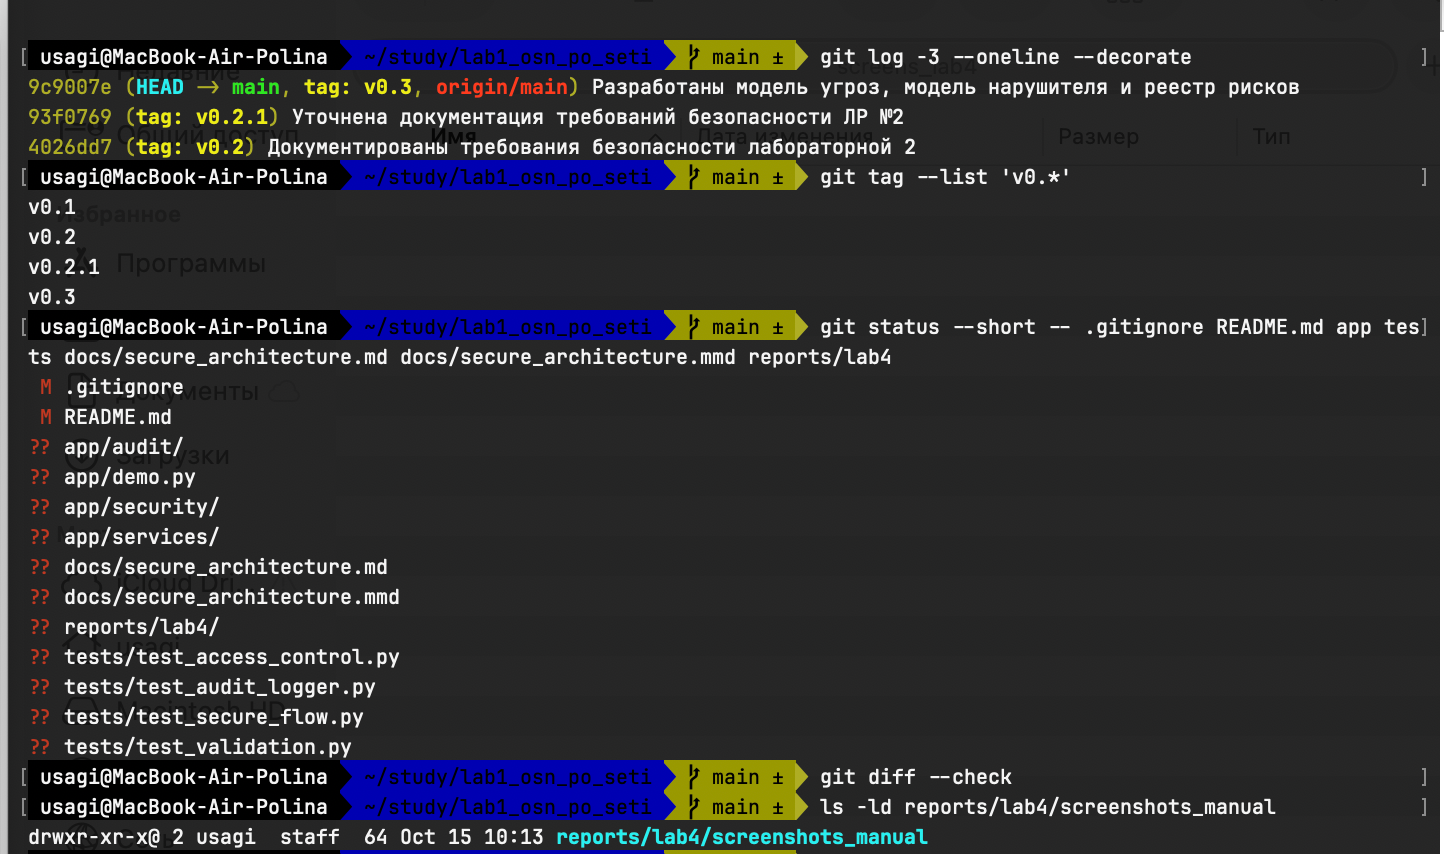
\includegraphics[width=0.97\linewidth,height=0.62\textheight,keepaspectratio]{screenshots_manual/lab4_5_1.png}
\caption{История версий, подготовленные изменения и проверка diff до релиза.}
\end{figure}
\begin{figure}[H]
\centering
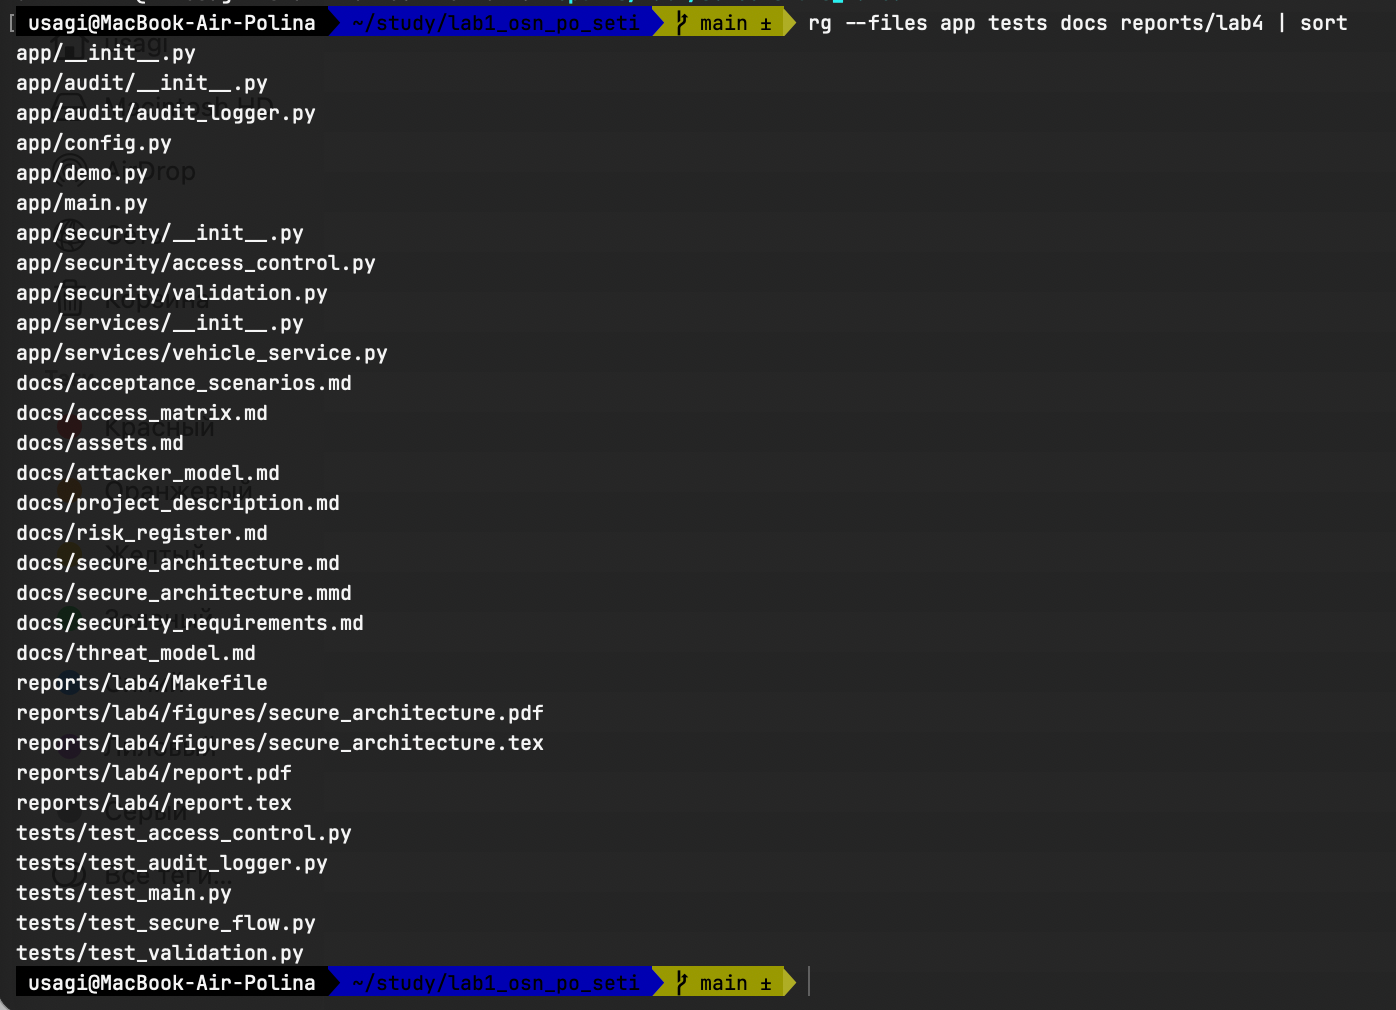
\includegraphics[width=0.97\linewidth,height=0.62\textheight,keepaspectratio]{screenshots_manual/lab4_5_2.png}
\caption{Структура исходников, документации и отчёта v0.4.}
\end{figure}

\section{Ответы на контрольные вопросы}
\begin{enumerate}
\item Архитектура - структура основных частей программы и правил их взаимодействия. Здесь поток проходит от интерфейса через проверки и сервис к данным.
\item Обычная архитектура описывает устройство, защищённая дополнительно учитывает нарушителей, границы доверия, полномочия, отказ и аудит.
\item Secure by Design означает учитывать защиту при выборе структуры и интерфейсов с самого начала, например проверять право до изменения записи.
\item Defense in Depth - несколько независимых слоёв контроля: валидация, авторизация, ограниченное хранилище и аудит.
\item Минимальные привилегии дают субъекту только права, нужные его задаче; водитель не меняет состояние ТС.
\item Доверительная граница - место перехода между зонами с разным уровнем доверия, например клиент к приложению (\texttt{TB-01}).
\item Данные на границе могут быть изменены или ошибочны, поэтому тип, размер, диапазон и право на объект проверяются до операции.
\item Точка входа - интерфейс, через который данные или действия попадают в систему; пример сейчас - CLI, в будущем - веб-форма.
\item Поверхность атаки - совокупность доступных точек входа, операций, компонентов и зависимостей, которыми можно злоупотребить.
\item Разделение интерфейса, логики и хранилища не позволяет обходить правила сервиса прямой работой клиента с данными и облегчает независимую проверку.
\item Аутентификация устанавливает, кто субъект; авторизация решает, разрешено ли ему конкретное действие над объектом.
\item Неизвестная роль не имеет доказанных полномочий; автоматическое разрешение превращает ошибку в выдачу доступа, поэтому применяется deny by default \cite{owasp-asvs,owasp-auth}.
\item Fail Secure означает при ошибке завершить операцию безопасным отказом, не открывая доступ и не оставляя частичное изменение.
\item Журналируют вход/отказ, изменение ролей и учётных данных, операции с поездками и значимые ошибки валидации.
\item Нельзя писать пароли, токены, \texttt{APP\_SECRET\_KEY}, ключи, секретные поля и избыточное содержимое маршрутов.
\item Модель угроз помогает выбрать контроль для конкретного сценария до закрепления архитектуры, иначе границы и данные могут быть спроектированы без необходимой проверки.
\item Остаточный риск - риск, остающийся после выбранных мер; он не равен нулю только потому, что отдельный тест прошёл.
\item Связь показывает, какой компонент и контроль прерывает шаг угрозы, и какие условия всё ещё позволяют ей реализоваться.
\end{enumerate}

\section{Вывод}
В v0.4 создан компактный прототип с предметной валидацией, проверкой ролей и владельца поездки, сервисом смены статуса и безопасным форматом аудита. Все 45 автоматических тестов и CLI-демонстрация подтвердили перечисленные свойства учебного стенда. Аутентификация, СУБД, сетевой API и долговременное хранилище остаются проектными. Настоящие скриншоты выполнения команд включены в разделы тестирования и Git.

\clearpage
\renewcommand{\refname}{Список использованных источников}
\addcontentsline{toc}{section}{Список использованных источников}
\begin{thebibliography}{99}
\bibitem{method4} Методические указания «Практическая работа № 4. Проектирование защищённой архитектуры приложения».
\bibitem{nist-ssdf} Souppaya M., Scarfone K., Dodson D. Secure Software Development Framework (SSDF) Version 1.1: Recommendations for Mitigating the Risk of Software Vulnerabilities. NIST SP 800-218. Gaithersburg: National Institute of Standards and Technology, 2022. URL: \url{https://csrc.nist.gov/pubs/sp/800/218/final} (дата обращения: 15.10.2026).
\bibitem{owasp-asvs} \mbox{OWASP} Foundation. Application Security Verification Standard (ASVS), version 5.0.0 [Электронный ресурс]. URL: \url{https://owasp.org/www-project-application-security-verification-standard/} (дата обращения: 15.10.2026).
\bibitem{owasp-auth} \mbox{OWASP} Foundation. Authorization Cheat Sheet [Электронный ресурс]. URL: \url{https://cheatsheetseries.owasp.org/cheatsheets/Authorization_Cheat_Sheet.html} (дата обращения: 15.10.2026).
\end{thebibliography}
\end{document}
